\documentclass[a6paper,10pt]{article}
%\usepackage[T1]{fontenc}
\usepackage[british]{babel}
\usepackage[utf8]{inputenc}
\usepackage{float, graphicx,amsmath,amsfonts,cite,enumerate}
\usepackage[final]{pdfpages}
\usepackage{wrapfig}
\usepackage[margin=0.3in]{geometry}
\usepackage{sidspaltHack}

\newcommand{\mel}[1]{\small\textbf{\textit{mel. #1 \\}}}


\setlength{\oddsidemargin}{-0.37in}
\setlength{\textwidth}{215pt}

\pagestyle{empty}

\begin{document}
\nysida{3}{1}
\noindent
\huge{$\Gamma\gamma$ Visor till öl}
\begin{center}
\Large $\gamma1$. Ölbytarvisan \\ 
\mel{Kgl Södermanlands Regementes marsch}
\end{center}
\small Här i Bayern skall ölet flöda fritt. \\
Ingen skiljer här nå'nsin mellan mitt och ditt. \\
Bjud varandra så håller ni er kvitt. \\
Saknar någon en öl, \\
får hen en utan men. \\
\newline
Raj-raj... \\
\newline
Gillar du öl \\
så ge din granne en öl. \\
Tar hen din öl \\
så får du nog hens öl. \\
Båda har öl \\
och ni har båda blivit bjudna. \\
Så ni har det bra \\
tills ni ser sejdelbottnarna! 
\begin{flushright}
\textit{Fysikalen Wagner 1986}
\end{flushright}

\nysida{3}{2}
\setlength{\oddsidemargin}{-0.47in}
\begin{center}
\Large $\gamma2$. Strejk på Pripps \\ 
\mel{I natt jag drömde}
\end{center}
I natt jag drömde något som\\
jag aldrig drömt förut.\\
Jag drömde det var strejk på Pripps\\
och alla ölen var slut.
\vspace{5pt}\\
Jag drömde om en jättesal\\
där ölen stod på rad.\\
Jag drack så där en femton öl\\
och reste mig och sa:
\vspace{5pt}\\
"En kan ha roligt utan sprit\\
Men det är dumt att chansa!"
\begin{center}
\Large $\gamma3$. Ode till ölet \\ 
\mel{Trampa på gasen}
\end{center}
Tu-tu-tu Tuborg\\
och ca-ca-ca Carlsberg\\
det är den bästa \\
pi-pi-pi pilsnern som jag vet.
\vspace{5pt} \\
Tu-tu-tu Carlsberg\\
och ca-ca-ca Tuborg\\
det är det bästa\\
pi-pi-pi ölet som jag vet.
\vspace{5pt} \\
Tu-tu-tu Ölberg\\
och ca-ca-ca Pilsborg\\
det är den bästa \\
pi-pi-pi biran som jag vet!
\vspace{5pt}\\
Tu-ca-pi Ölsner och \\
pi-tu-ca bira\\
det är den mästa ca-pi-tu-lering som jag gjort.

\nysida{3}{4}
\setlength{\oddsidemargin}{-0.37in}
\begin{center}
\Large $\gamma4$. Min pilsner \\ 
\mel{My Bonnie}
\end{center}
Min pilsner skall svalka min tunga. \\
Min pilsner skall duscha min gom. \\
Min pilsner skall få mig att sjunga, \\
om jag ser att flaskan är tom: \\
\newline
PILSNER! PILSNER! \\
Hämta en pilsner till mig, till mig. \\
PILSNER! PILSNER! \\
Hämta en pilsner till mig!
\vspace{40pt}
\begin{center}
\Large $\gamma5$. Sanningen om ölet \\ 
\mel{Här är gudagott att vara}
\end{center}
Gudagott är ölen på fat. \\
O, vad öldrycken dock är skön. \\
Dricka öl med älskad kamrat. \\
Billigare än likören grön. \\
Humlan surrar, vännen strålar. \\
Nu går jag och slår en drill. \\
Lättad, törstig, sedan jag skålar \\
i gott öl vännen min till. 

\nysida{3}{6}
\setlength{\oddsidemargin}{-0.47in}
\begin{center}
\Large $\gamma6$. Ölvisan \\ 
\mel{SJ, SJ, gamle vän}
\end{center}
Dricka pilsner varje da'\\
de e kul å de e bra.\\
Ja, det borde alla ha,\\
pilsner varje da.
\vspace{5pt}\\
Öl det slinker ner så lätt\\
lättare än fläskkotlett.\\
Å när en har slunkit ner\\
så måste du ha fler.
\vspace{5pt}\\
Efter sex, sju flaskor till\\
blir det svårt att sitta still.\\
Å vid cirka trettitvå\\
blir det svårt att gå.
\vspace{5pt}\\
Öl de e ju faktiskt mat\\
öl på burk å öl på fat.\\
Måste fyllas på i ett\\
för annars går det snett.
\vspace{5pt}\\
Ingen har väl illa mått\\
utav öl som är så gott.\\
Den som ändå detta gjort\\
har druckit det för fort.
\vspace{5pt}\\
Så korka upp din öl å drick\\
så blir du en festlig prick.\\
Korka upp å drick min vän\\
och rapa högljutt sen.

\nysida{3}{7}
\setlength{\oddsidemargin}{-0.37in}
\begin{center}
\Large $\gamma7$. En pilsnerdrickare \\ 
\mel{En sockerbagare}
\end{center}
En pilsnerdrickare här bor i staden\\
hen dricker pilsner mest hela dagen\\
hen dricker gröna, hen dricker blå,\\
hen dricker några med renat på.\\
Och i hens fönster hänga tomma glasen,\\
och alla burkarna från kalasen\\
och är hen nykter så kan hen gå\\
nertill butiken och fylla på.
\begin{figure}[!h]
\hspace{30pt}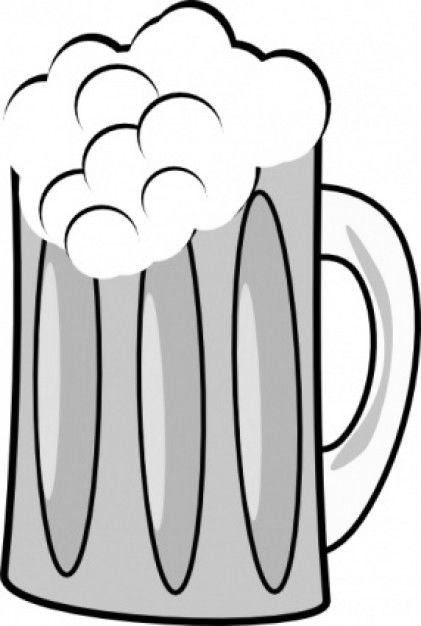
\includegraphics[width=0.3\textwidth]{ol.jpg}
\end{figure}
\begin{center}
\Large $\gamma8$. Öl, öl, öl i glas \\ 
\mel{Row, row, row your boat}
\end{center}
Öl, öl, öl i glas eller i butelj.\\
Skummande, skummande, skummande, skummande.\\
Ta en klunk och svälj.

\nysida{3}{9}
\setlength{\oddsidemargin}{-0.47in}
\begin{center}
\Large $\gamma9$. Lapin Kulta\\ 
\mel{Broder Jakob}
\end{center}
Lapin Kulta, Lapin Kulta\\
Karjala, Karjala\\
Aura sekä Olvi, Aura sekä Olvi\\
Koff, Koff, Koff\\
Koff, Koff, Koff
\begin{center}
\Large $\gamma10$. Ju mera öl vi dricker\\ 
\mel{Ju mer vi är tillsammans}
\end{center}
Ju mera öl vi dricker,\\
vi dricker, vi dricker,\\
ju mera öl vi dricker,\\
ju rundare vi bli.
\vspace{5pt} \\
För rundare är sundare\\
och sundare är rundare.\\
Ju mera öl vi dricker,\\
ju rundare vi bli.
\begin{center}
\Large $\gamma11$. Vi älskar öl \\ 
\mel{Ser du stjärnan i det blå}
\end{center}
Täckt av silver sejdeln full\\
gnistrar mot oss med sitt guld\\
humle, malt, är livets salt, vi älskar öl. 
\vspace{5pt}\\
Källarsval så bärs den in\\
för att glädja gommen din\\
släcka törsten, stärka rösten, till dess lov. 
\vspace{5pt}\\
Knubbig blir du, men so what\\
gott och roligt har du fått\\
extra turen, rensat njuren, öl är gott.
\end{document}